\documentclass[conference]{IEEEtran}
% \IEEEoverridecommandlockouts
% The preceding line is only needed to identify funding in the first footnote. If that is unneeded, please comment it out.
\usepackage{cite}
\usepackage{amsmath,amssymb,amsfonts}


\usepackage{hyperref}
%\usepackage[ngerman]{cleveref}
\usepackage[english]{cleveref}

% \usepackage{algorithmic}
\usepackage{graphicx}
\usepackage{textcomp}
\usepackage{xcolor}
\def\BibTeX{{\rm B\kern-.05em{\sc i\kern-.025em b}\kern-.08em
    T\kern-.1667em\lower.7ex\hbox{E}\kern-.125emX}}
\begin{document}

\title{Text Analytica: cloud-based document analysis\\}

\author{\IEEEauthorblockN{Florian x}
\IEEEauthorblockA{\textit{Department of Computer Science} \\
\textit{University of Bristol}\\
Bristol, United Kingdom \\
ya18048@bristol.ac.uk}
\and
\IEEEauthorblockN{Nathalie Pett}
\IEEEauthorblockA{\textit{Department of Computer Science} \\
\textit{University of Bristol}\\
Bristol, United Kingdom \\
aq18034@bristol.ac.uk}
}

\maketitle

\begin{abstract}
The application can be run online at http://textanalytics.lukaspman.io/.
The source code is available at https://github.com/darkcookie298/CloudComputing.
\end{abstract}

\section{Introduction}
\label{sec:intro}
Text Analytica is a cloud-based application which aims to support the analysis of text documents. For the purpose of this coursework a prototype has been developed and deployed using different cloud computing technologies. In the remainder of this \cref{sec:intro}, the general concept behind Text Analytica is discussed as well as the limitations of the implemented prototype. The \cref{sec:platform-choice} of this report explores the reasons behind choosing Microsoft’s cloud services over Oracle’s. Afterwards in \cref{sec:system-architecture} the system architecture and technologies used for the project are explained in more detail. The scalability of the developed solution is addressed in \cref{sec:scalability}, including evidence of the performance of the service under load. Lastly, in \cref{sec:future-improvments}, future improvements of the application are proposed.

\begin{figure*}[ht!]
%\centering
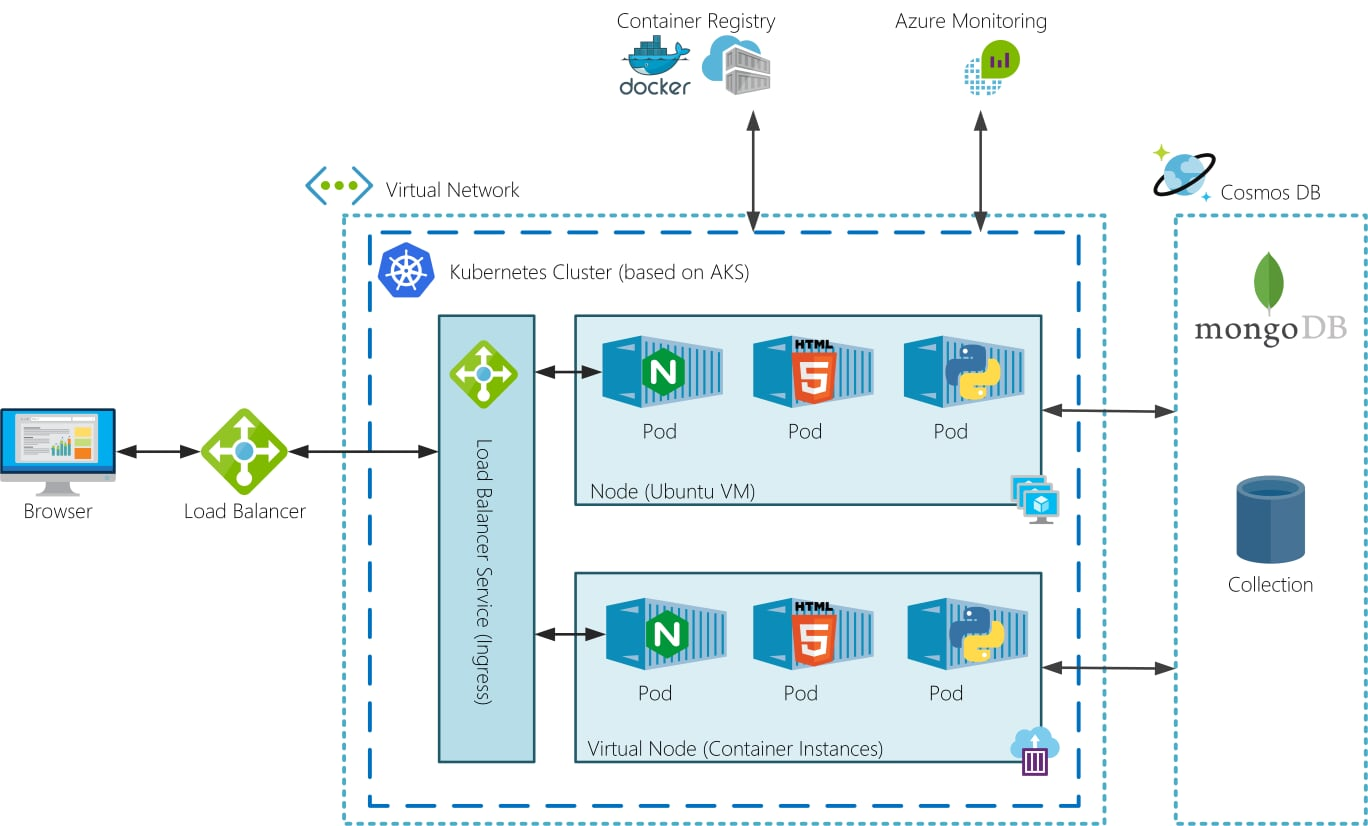
\includegraphics[width=150mm]{img/architecture.jpeg}
\caption{System architectue of our Kubernetes cluster.}
\label{img:architecture}
\end{figure*}

\subsection{Vision}
University students are often faced with an abundance of resources regarding specific units or even certain topics within a unit. These range from lecture notes or slides to personal notes and additional scientific papers as well as e-books or extracts thereof. The first step in the exploration process is for students to familiarise themselves with these materials by identifying the documents’ key aspects and discovering links between different sources. This is what Text Analytica ultimately aims to facilitate.

More specifically the functionalities of Text Analytica could include tagging, keyword search, suggestions of related documents based on textual analysis and eventually the generation of short summaries, all based on user-supplied PDF documents. These functionalities render Text Analytica a useful tool for a large number of scenarios in which people are confronted with many different and possibly complex text sources, e.g. in the context of management decisions in industry or business / commerce.

\subsection{Limitations of the submitted prototype}
The focus of this coursework assignment was to deploy an application using different cloud services and explore its scalability. Therefore the functionality of the submitted Text Analytica prototype was stripped down to a minimum.

To skip the step of extracting machine readable text from PDFs by applying OCR techniques, currently users are only able to upload simple .txt documents. These files are then parsed and analysed. At this point the analysis merely tags the system entries with the three most used words in the text. As the current state of analysis functionality does not require the files to be stored within the application, they are discarded after being processed. Additionally the user account and login functionality has not yet been implemented.

\begin{itemize}
	\item explain what we actually implemented and how it is different from the proposed application in FA2 (point to section about improvements)
\end{itemize}

\section{Platform choice}
\label{sec:platform-choice}
The considerations detailed below led to choosing to work with Microsoft Azure to remain within the given time scope for the coursework.
\subsection{Setup}
\begin{itemize}
	\item technical issues with Oracle: unintuitive UI (add contributor), service limits
\end{itemize}

At first we tried to use the Oracle Cloud and to build and maintain a kubernetes cluster we wanted to use the Terraform command
line tool. This was the recommended way we got from the tutorials in class from the Orcale Team.
After a long period of installing all needed tools e.g. \textit{Terraform} itself, \textit{Terraform Provider},
\textit{Terraform Kubernetes Installer for Oracle Cloud} \cite{TerrafromK8sInstaller}, we tried to create an easy example cluster.
But already at this point we run into service limits. These limits are restrictions on how many instances of a specific resource you are
allowed to use. To increase the limit you have to open a ticket request and than after a few days there will be an Oracle support guy
helping you. As the ticket request system is very inconvienient and complicated, and the whole process takes several days this is a very strong
disadvantage of the \textbf{Oracle Cloud} in comparison to \textbf{Microsoft's Azure}.

\subsection{Documentation and support}
An even bigger advantage of using one of \textit{"the big three"}, so Google Cloud, Amazon AWS or Microsoft Azure, is there are
a lot of tutorials, answered questions on \textit{Stackoverflow},etc and better documentations. Respectively using Oracle leads to
a very small number of tutorials, which is one of the reasons why it is more difficult for beginners. There were a lot of errors, too,
but searching for solutions of our problems with Terraform and Oracle Cloud was very unsuccessfull.
So after increasing the service limits and running in errors again and again, we got to a point, where we decided to switch to Azure.
In retrospect this was one of our best decisions of the whole project.

\begin{itemize}
	\item more documentation
	\item more community support
\end{itemize}

\subsection{More Advantages}
\begin{itemize}
	\item faster scaling without the need of starting a new VM for peak times
	\item TODO add other more 'small' advantages
\end{itemize}

\section{System architecture}
\label{sec:system-architecture}
\subsection{Infrastructure}
\begin{itemize}
	\item container and Kubernetes (IaaS)
\end{itemize}

\subsection{Data storage}
\begin{itemize}
	\item CosmosDB (PaaS); similar to MongoDB: high availability, scaling, ...
\end{itemize}

\subsection{Microservices}
\begin{itemize}
	\item Flask and 3rd party
	\item REST API between front end and back end,  services (back end, analysis, front end)
\end{itemize}

\subsection{Infrastructure as code}
\begin{itemize}
	\item infrastructure can be deployed from a template automatically
\end{itemize}

\section{Scalability}
\label{sec:scalability}
\subsection{Infrastructure}
As mentioned in \cref{sec:system-architecture} all services are managed by the Kubernetes cluster.
The main advantage of using a Kubernetes cluster is scailability and loadbalancing. So if there is a high usage of the
existing ressources the cluster can scale up by itself. In our case this might happen at peak times when a lot of people
are using the Text Analytica webservice. Than the cluster creates more (TODO:  describe more carefully what exactly happens here)
\cite{MicrosoftAzureKubernetesService}.

As we are using the Azure specific option of \textit{Virtual Nodes}, we can achieve even faster up- and downscaling times
than with the pure Kubernetes cluster itself. This is due to the fact we do not need to wait on new VMs or container booting up (TODO: check this).
\cite{MicrosoftVirtualNode}.

\subsection{Data storage}
\begin{itemize}
	\item PaaS and other region
\end{itemize}

\subsection{Service}
\begin{itemize}
	\item container and microservices -> why is this important for scalability?!
\end{itemize}

\subsection{Monitoring and Load Testing}
\begin{itemize}
	\item include some evidence on how our application scales
	\item maybe show screenshots and explain functionality of kubernetes dashboard
\end{itemize}

\section{Future improvements}
\label{sec:future-improvments}
\subsection{Infrastructure}
\begin{itemize}
	\item serverless (Lambda, Azure functions),  PaaS
\end{itemize}

\subsection{Service}
\begin{itemize}
	\item add functionality (login, pdf, text recognition, more advanced analysis, save files and retrieve them, ...)
	\item better scoping of microservices
	\item use of more Kubernetes functionalities
\end{itemize}

\subsection{Monitoring}
\begin{itemize}
	\item advanced cloud monitoring
\end{itemize}

\section{Conclusion}
\label{sec:conclusion}
conclusion...

\bibliographystyle{acm}

%\nocite{*}
\bibliography{cw1-97059-97133}


\end{document}
